\chapter{Methodology}
This chapter covers the various methodologies that were implemented in this project. It takes a look at the different types of research methodologies that were used such as ..., the different types of software development methodologies that were used such as ..., and why each was chosen. Other areas also covered in this chapter include meetings, project management, development tools, source control, and testing.

\section{Research Methodology}
The research methodology that was used in this project was Qualitative Research. Qualitative research approaches are employed across many academic disciplines and is useful at an individual level. Qualitative data collection methods vary using unstructured or semi-structured techniques.

\section{Software Development Methodology}
The software development methodology that was used in this project was Extreme Programming (XP). Extreme Programming is a software development methodology designed to improve the quality of software and its ability to properly adapt to the changing needs of the customer or client. While there was no customer or client for this project, this methodology was still applicable. 
\par
\medskip
It is a form of Agile software development. The Agile methodology was developed as a response to growing frustrations with Waterfall and other highly structured, inflexible methodologies. This approach is designed to accommodate change and the need to produce software faster. Similar to other Agile methods of development, Extreme Programming aims to provide iterative and frequent small releases throughout the project, allowing both team members and customers to examine and review the project’s progress throughout the entire SDLC (Software Development Life Cycle). 
\par
\medskip
It became clear early on that the Agile methodology would be the most suitable methodology to use for this project as the Agile Methodology allows for incremental development, changing requirements, prototyping, and sustainable development. As there would be weekly meetings with the project supervisor, being able to show and discuss the progress of the project would be a bonus. 

\section{Meetings}
Project meetings were held weekly for the duration of the project with the project supervisor. The majority of the meetings consisted of:
\begin{itemize}
    \item Project progress updates.
    \item Feedback on progress.
    \item Planning of the next development iteration.
    \item Discussions on possible additional features that could be incorporated.
    \item Q&A on various project elements.
\end{itemize}
\par
\medskip
Initial project meetings were more focused on brainstorming possible projects that could be developed. The first ... weeks comprised of research, whereby possible projects ideas, appropriate technologies, and a project timeline were developed.

\section{Project Management}

\section{Development Tools}
The main Integrated Development Environment used throughout the project was Visual Studio Code.

\section{Source Control}
Source control (or version control) is the practice of tracking and managing changes to code. GitHub provides hosting for software development version control using Git. Git is an open-source distributed source code management system.

\paragraph{Benefits of Git}
\subparagraph{Distributed Development}
Git is a distributed version control system. Instead of a working copy, each developer gets their own local repository, complete with a full history of commits. Having a full local history makes Git fast, since it means you don’t need a network connection to create commits, inspect previous versions of a file, or perform diffs between commits.

\subparagraph{Faster Release Cycle}


\section{Testing}
The main type of software testing development process used throughout the project was Test-driven development (TDD). Several different types of testing was used throughout in conjunction, such as Integration Testing, Unit Testing, System Testing, Performance Testing, etc. Several tools were used to aid in this, which included Postman, 

\centering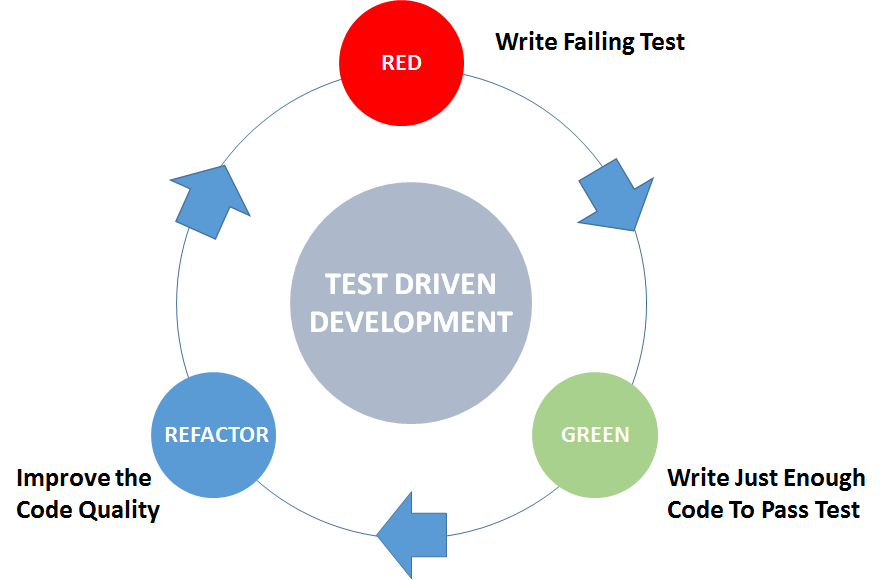
\includegraphics[width=8cm,height=3.3cm,keepaspectratio]{images/tdd}
